%
\clearpage
%
\section{Appendix}\label{sec:appendix}
The appendix presents two supporting examples covered in the two subsections below.  The first example demonstrates how LCBs are computed.  The second example illustrates the interdependence of LCBs.

\subsection {Example LCB Calculation}\label{sec:example_lcb_calculation}
To illustrate our approach for computing LCBs, consider the following example.  Assume we have two tasks, \begin{math}\tau_{1}\end{math} and \begin{math}\tau_{2}\end{math} with UCBs and ECBs for each listed in Figure~\ref{fig:taskset_ecbs_ucbs}.  Please note that we have not shown the ECBs, UCBs, or AUCBs in the following figures for $\delta_i^0$ as it is a dummy basic block with no elements for each of the aforementioned sets.
\vspace{-5pt}
\begin{figure}[h!]
\begin{center}
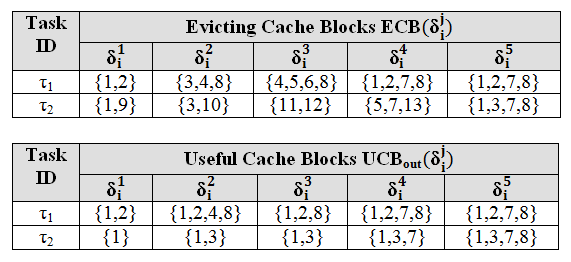
\includegraphics[width=\linewidth]{taskset_ecbs_ucbs.png}
\caption{Taskset ECBs and UCBs.}
\label{fig:taskset_ecbs_ucbs}
\end{center}
\end{figure}
\vspace{-10pt}
\newline
\noindent
The computation for LCBs uses the accessed useful cache blocks (AUCBs) since the cache blocks that are re-loaded during execution of the non-preemptive region between preemption points is a function of the memory that is explicitly accessed by the preempted task.  The computed AUCBs for each task is shown in Figure~\ref{fig:taskset_aucbs}. In accordance with Equation 7 one can readily see that the AUCBs are simply the intersection of the UCBs and ECBs for each basic block.
\vspace{-10pt}
\begin{figure}[h!]
\begin{center}
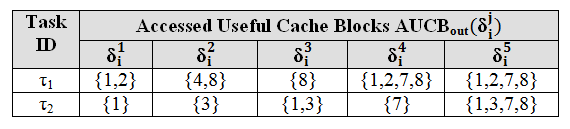
\includegraphics[width=\linewidth]{taskset_aucbs.png}
\caption{Taskset AUCBs.}
\label{fig:taskset_aucbs}
\end{center}
\end{figure}
\vspace{-10pt}
\newline
\noindent
In our example, assume preemptions are taken at basic blocks \begin{math}\delta_{1}^{2}\end{math} and \begin{math}\delta_{1}^{4}\end{math} for task \begin{math}\tau_{1}\end{math}. For simplicity, we calculate the LCBs associated with these two preemption points.  For $LCB(\delta_{1}^{2},\delta_{1}^{4})$, we have $UCB(\delta_{1}^{2})\ =\ \{1,2,4,8\}$.  The second expression is the set of memory that is accessed in basic blocks $\delta_{1}^{3}$ and $\delta_{1}^{4}$, namely $\{8\}\ \cup\ \{1,2,7,8\}\ =\ \{1,2,7,8\}$ comprising the set of AUCBs.  The third expression is the set of ECBs for task $\tau_{2}$ where $ECB(\tau_{2})\ =\ \{1,3,5,7,8,9,10,11,12,13\}$. Thus, $LCB(\delta_{1}^{2},\delta_{1}^{4})$ is given by the intersection of the three sets:
\begin{equation*}\label{eqn:lcb-example-1}
\begin{split}
    LCB(\delta_{1}^{2},\delta_{1}^{4}) = &\{1,2,4,8\}\ \cap\ \{1,2,7,8\}\ \cap\ \\&\{1,3,5,7,8,9,10,11,12,13\} = \{1,8\}
\end{split}
\end{equation*}
%\newline
\noindent
The preemption cost $\gamma(\delta_{1}^{2},\delta_{1}^{4})$ for a BRT = $390\mu$s is given by:
\begin{equation*}\label{eqn:gamma-example-1}
    \gamma(\delta_{1}^{2},\delta_{1}^{4}) = |\{1,8\}|\ \cdot\ 390 = 780\mu\textit{s}
\end{equation*}
%\newline
\noindent
Using the same method, $LCB(\delta_{1}^{4},\delta_{1}^{5})$ is given by:
\begin{equation*}\label{eqn:lcb-example-2}
\begin{split}
    LCB(\delta_{1}^{4},\delta_{1}^{5}) = &\{1,2,7,8\}\ \cap\ \{1,2,7,8\}\ \cap\ \\&\{1,3,5,7,8,9,10,11,12,13\} = \{1,7,8\}
\end{split}
\end{equation*}
%\newline
\noindent
The preemption cost $\gamma(\delta_{1}^{4},\delta_{1}^{5})$ for a BRT = $390\mu$s is given by:
\begin{equation*}\label{eqn:gamma-example-1}
    \gamma(\delta_{1}^{4},\delta_{1}^{5}) = |\{1,7,8\}|\ \cdot\ 390 = 1170\mu\textit{s}
\end{equation*}
%\newline
\noindent
Using the method illustrated here, the preemption cost matrix entries for each pair of basic blocks are computed in a similar fashion and used as input to our preemption point placement algorithm.
%
%\vspace{-20pt}
%\begin{figure}[h!]
%\begin{center}
%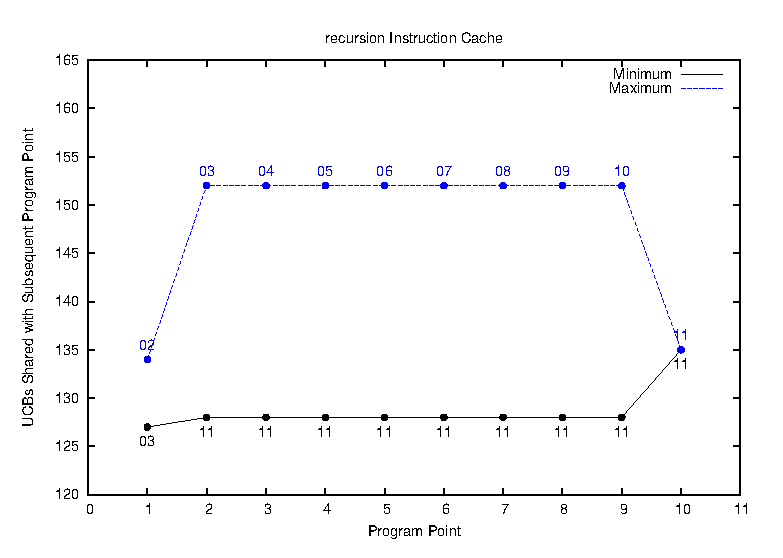
\includegraphics[width=\linewidth]{eps/recursion-icache.eps}
%\caption{Recursion Instruction Cache.}
%\label{fig:recursion_instruction_cache}
%\end{center}
%\end{figure}
%
%\vspace{-20pt}
%\begin{figure}[h!]
%\begin{center}
%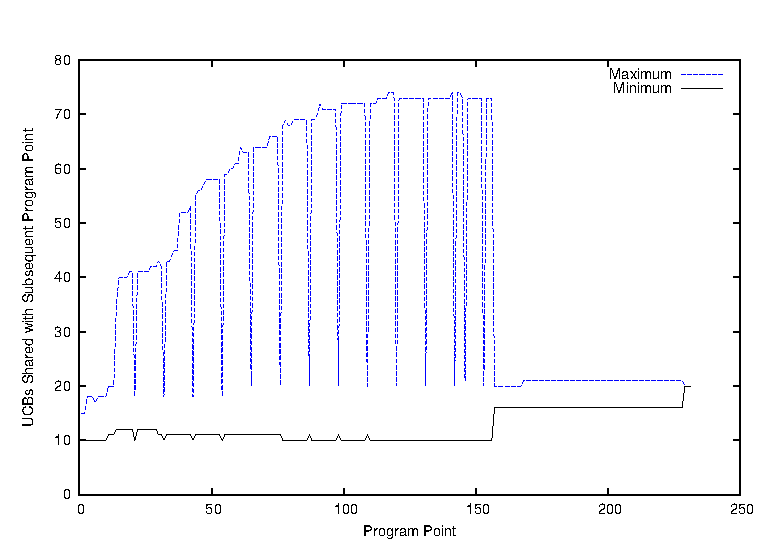
\includegraphics[width=\linewidth]{eps/adpcm-dcache.eps}
%\caption{ADPCM Data Cache.}
%\label{fig:adpcm_data_cache}
%\end{center}
%\end{figure}
%
%\vspace{-20pt}
%\begin{figure}[h!]
%\begin{center}
%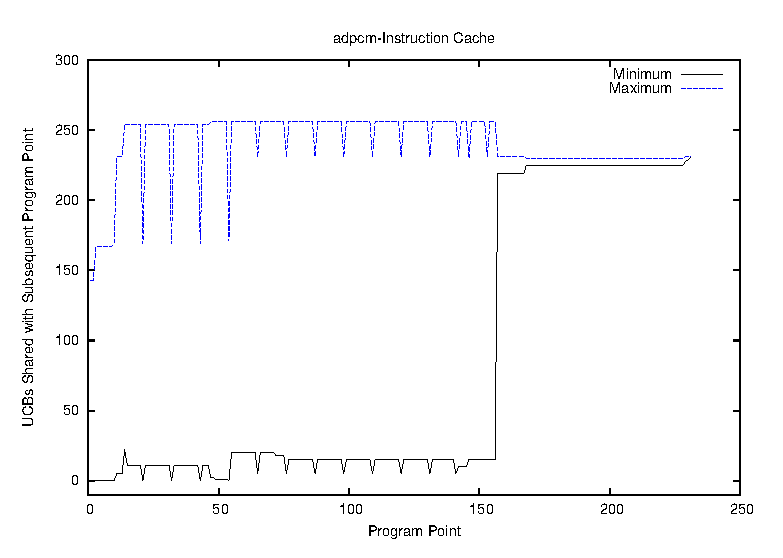
\includegraphics[width=\linewidth]{eps/adpcm-icache.eps}
%\caption{ADPCM Instruction Cache.}
%\label{fig:adpcm_instruction_cache}
%\end{center}
%\end{figure}
%
%\vspace{-20pt}
%\begin{figure}[h!]
%\begin{center}
%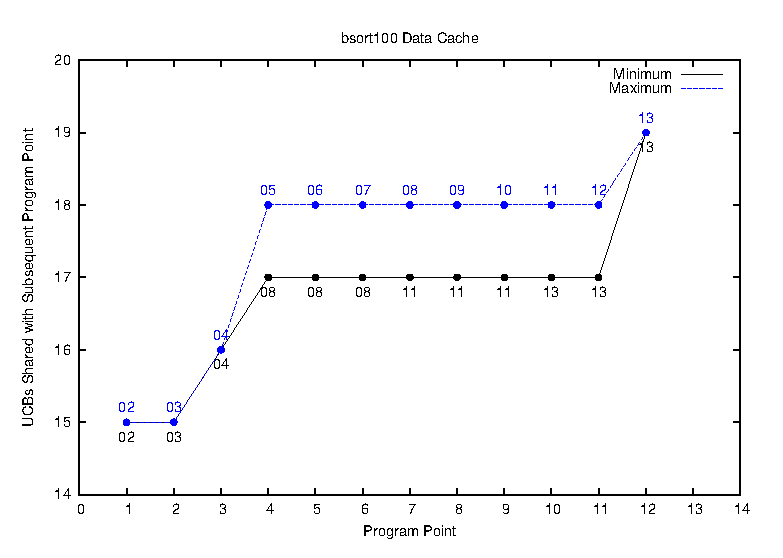
\includegraphics[width=\linewidth]{eps/bsort100-dcache.eps}
%\caption{BSORT100 Data Cache.}
%\label{fig:bsort100_data_cache}
%\end{center}
%\end{figure}
%
%\vspace{-20pt}
%\begin{figure}[h!]
%\begin{center}
%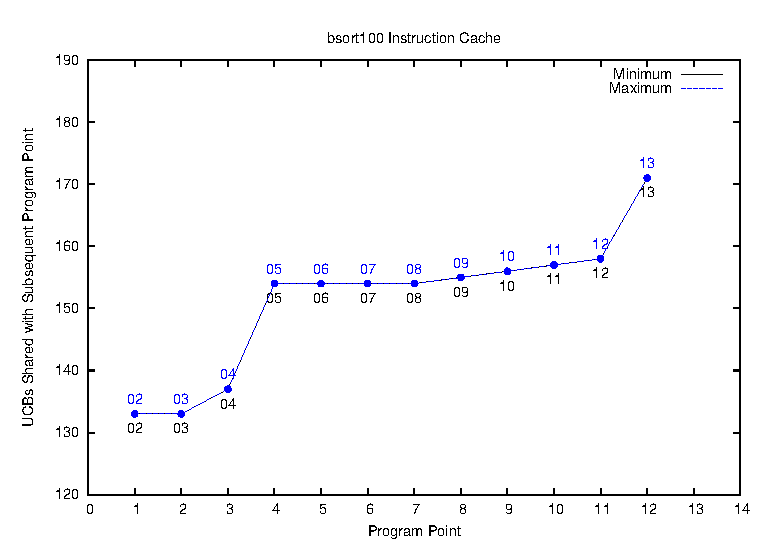
\includegraphics[width=\linewidth]{eps/bsort100-icache.eps}
%\caption{BSORT100 Instruction Cache.}
%\label{fig:bsort100_instruction_cache}
%\end{center}
%\end{figure}
%
%\vspace{-20pt}
%\begin{figure}[h!]
%\begin{center}
%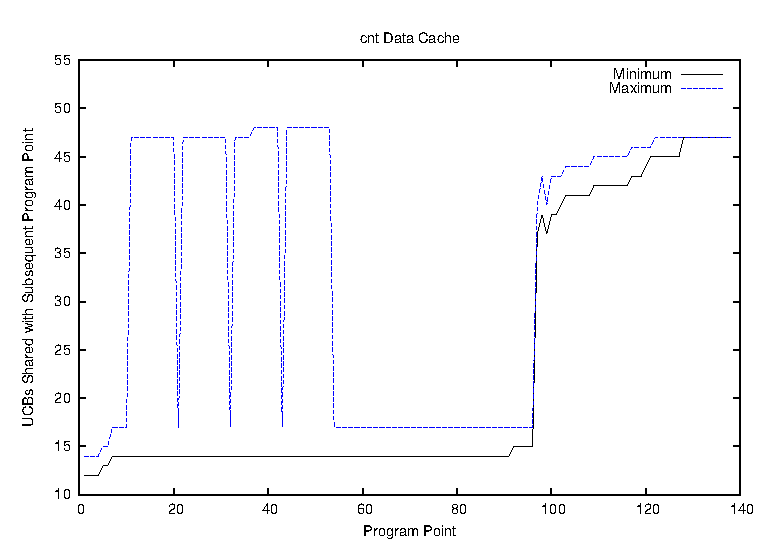
\includegraphics[width=\linewidth]{eps/cnt-dcache.eps}
%\caption{CNT Data Cache.}
%\label{fig:cnt_data_cache}
%\end{center}
%\end{figure}
%
%\vspace{-20pt}
%\begin{figure}[h!]
%\begin{center}
%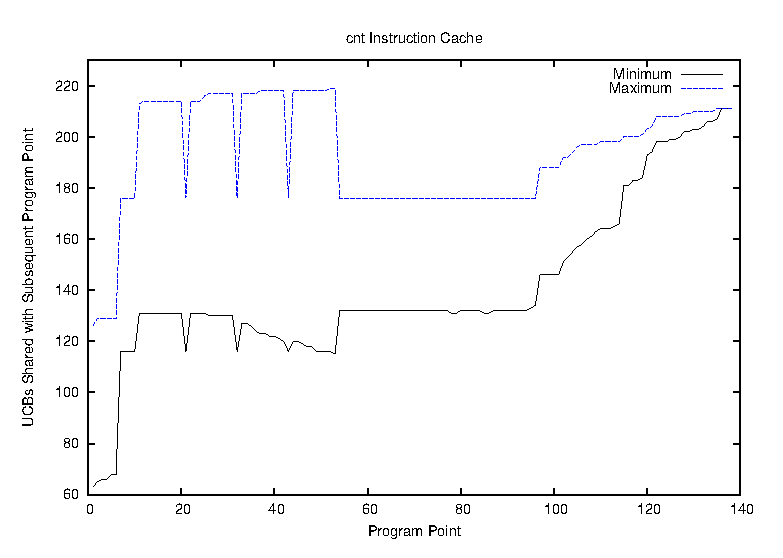
\includegraphics[width=\linewidth]{eps/cnt-icache.eps}
%\caption{CNT Instruction Cache.}
%\label{fig:cnt_instruction_cache}
%\end{center}
%\end{figure}
%
%\vspace{-20pt}
%\begin{figure}[h!]
%\begin{center}
%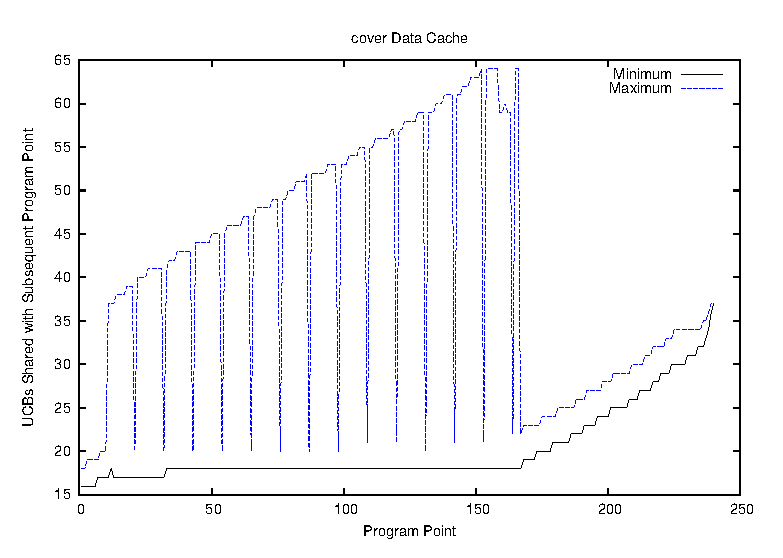
\includegraphics[width=\linewidth]{eps/cover-dcache.eps}
%\caption{Cover Data Cache.}
%\label{fig:cover_data_cache}
%\end{center}
%\end{figure}
%
%\vspace{-20pt}
%\begin{figure}[h!]
%\begin{center}
%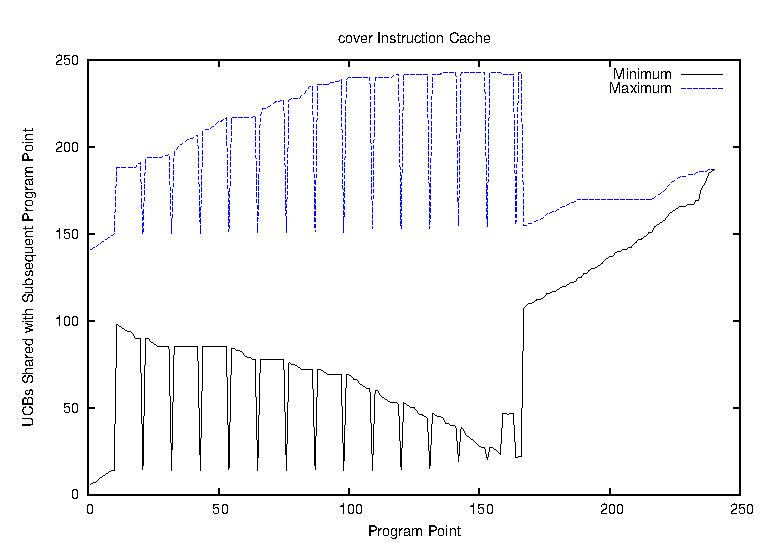
\includegraphics[width=\linewidth]{eps/cover-icache.eps}
%\caption{Cover Instruction Cache.}
%\label{fig:cover_instruction_cache}
%\end{center}
%\end{figure}
%
%\vspace{-20pt}
%\begin{figure}[h!]
%\begin{center}
%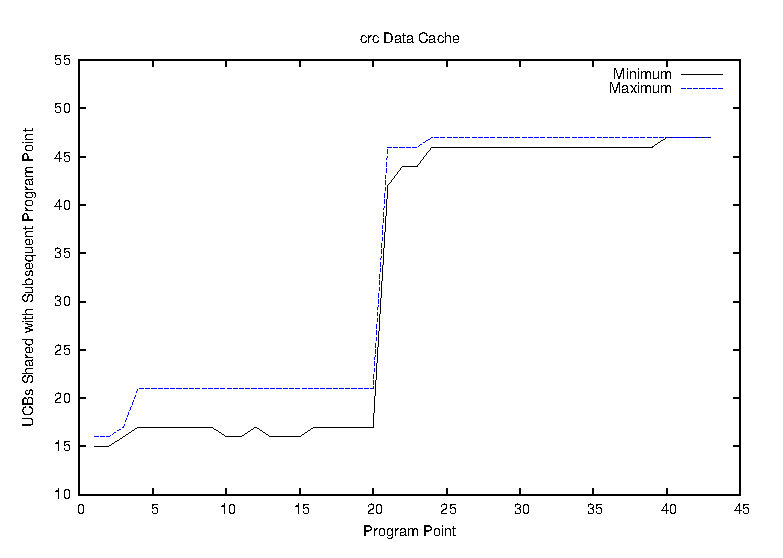
\includegraphics[width=\linewidth]{eps/crc-dcache.eps}
%\caption{CRC Data Cache.}
%\label{fig:crc_data_cache}
%\end{center}
%\end{figure}
%
%\vspace{-20pt}
%\begin{figure}[h!]
%\begin{center}
%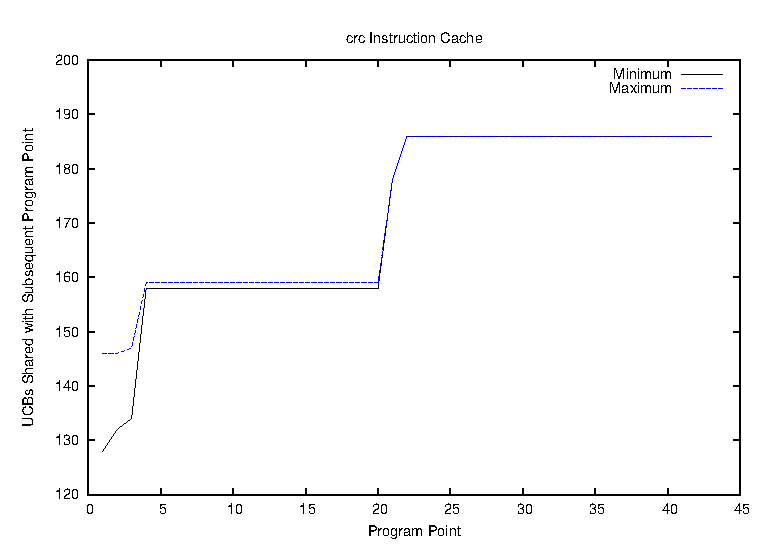
\includegraphics[width=\linewidth]{eps/crc-icache.eps}
%\caption{CRC Instruction Cache.}
%\label{fig:crc_instruction_cache}
%\end{center}
%\end{figure}
%
%\vspace{-20pt}
%\begin{figure}[h!]
%\begin{center}
%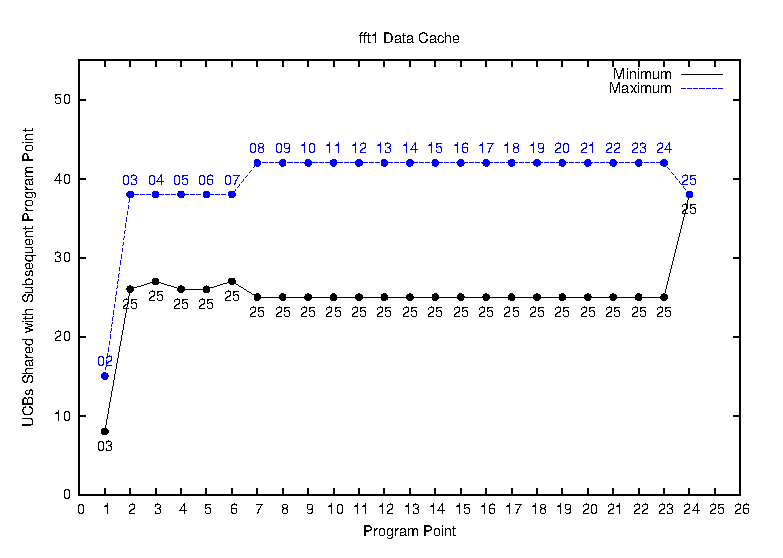
\includegraphics[width=\linewidth]{eps/fft1-dcache.eps}
%\caption{FFT1 Data Cache.}
%\label{fig:fft1_data_cache}
%\end{center}
%\end{figure}
%
%\vspace{-20pt}
%\begin{figure}[h!]
%\begin{center}
%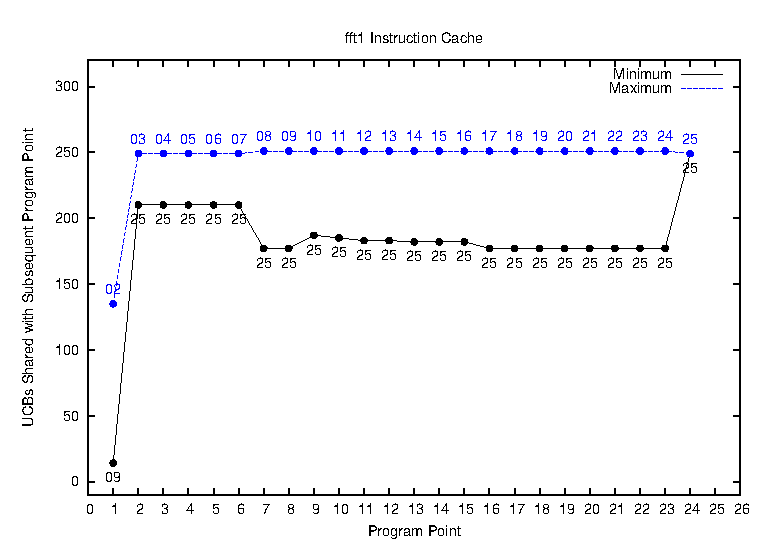
\includegraphics[width=\linewidth]{eps/fft1-icache.eps}
%\caption{FFT1 Instruction Cache.}
%\label{fig:fft1_instruction_cache}
%\end{center}
%\end{figure}
%
%\vspace{-20pt}
%\begin{figure}[h!]
%\begin{center}
%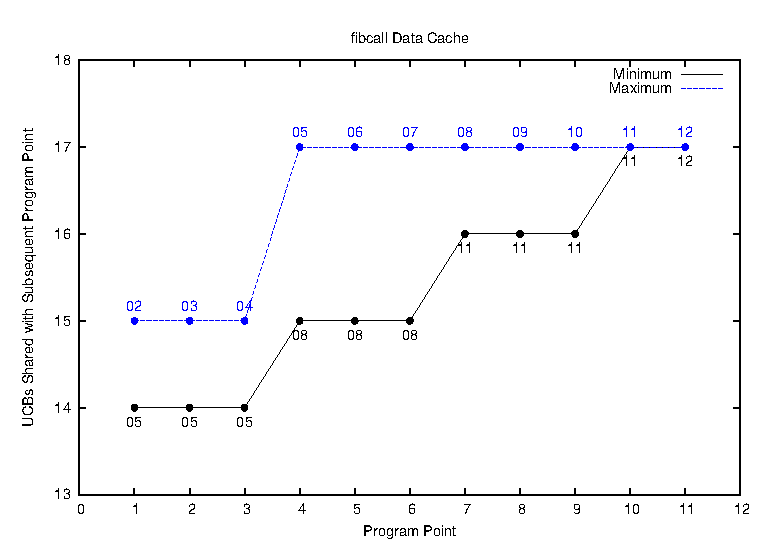
\includegraphics[width=\linewidth]{eps/fibcall-dcache.eps}
%\caption{Fibcall Data Cache.}
%\label{fig:fibcall_data_cache}
%\end{center}
%\end{figure}
%
%\vspace{-20pt}
%\begin{figure}[h!]
%\begin{center}
%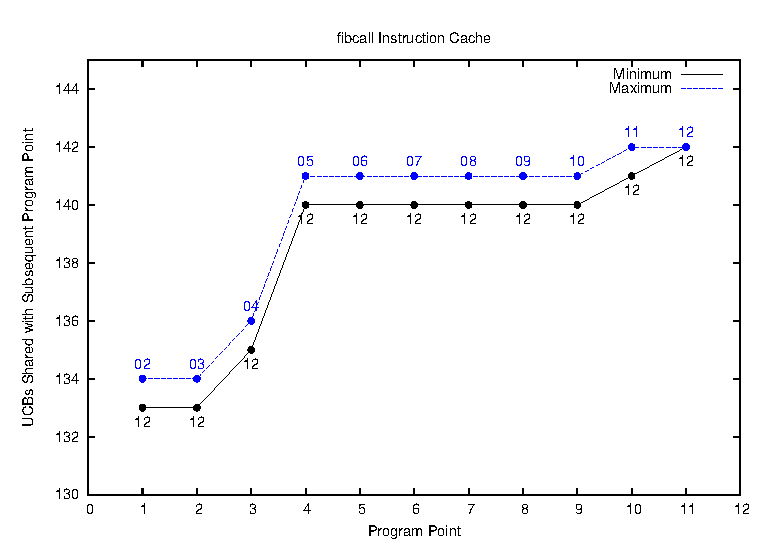
\includegraphics[width=\linewidth]{eps/fibcall-icache.eps}
%\caption{Fibcall Instruction Cache.}
%\label{fig:fibcall_instruction_cache}
%\end{center}
%\end{figure}
%
%\begin{figure}[h!]
%\vspace{-20pt}
%\begin{center}
%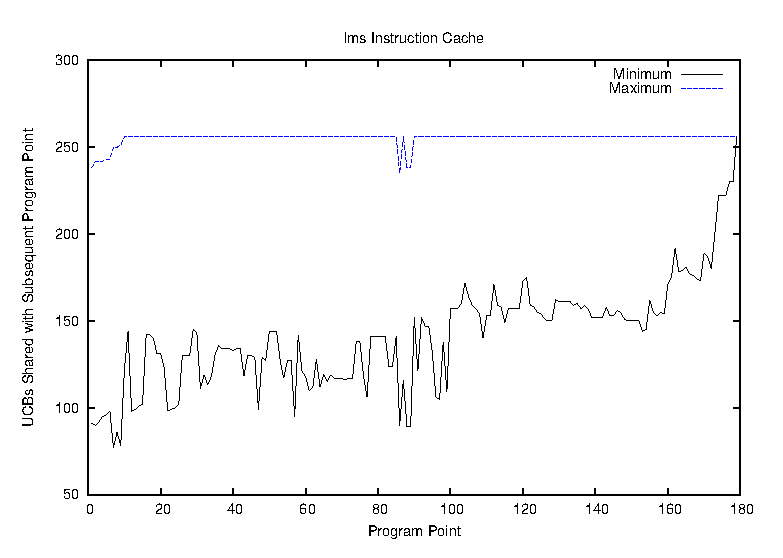
\includegraphics[width=\linewidth]{eps/lms-icache.eps}
%\caption{LMS Instruction Cache.}
%\label{fig:lms_instruction_cache}
%\end{center}
%\vspace{-10pt}
%\end{figure}
%
%\vspace{-20pt}
%\begin{figure}[h!]
%\begin{center}
%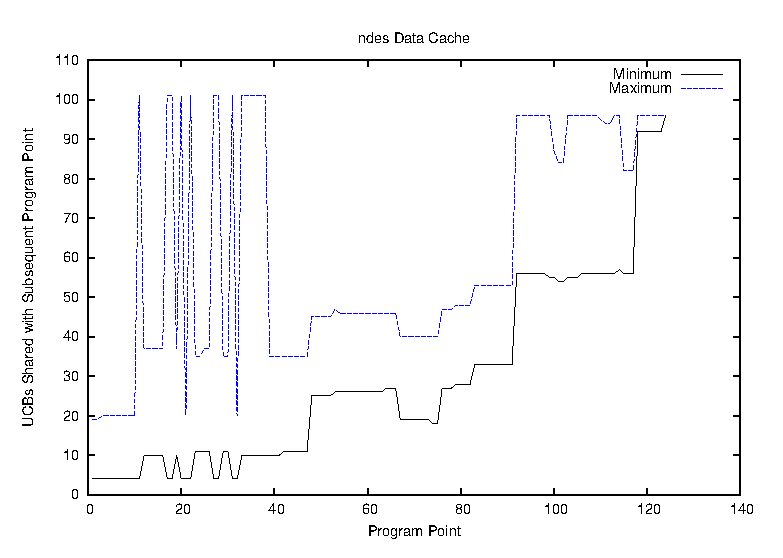
\includegraphics[width=\linewidth]{eps/ndes-dcache.eps}
%\caption{NDES Data Cache.}
%\label{fig:ndes_data_cache}
%\end{center}
%\end{figure}
%
%\vspace{-20pt}
%\begin{figure}[h!]
%\begin{center}
%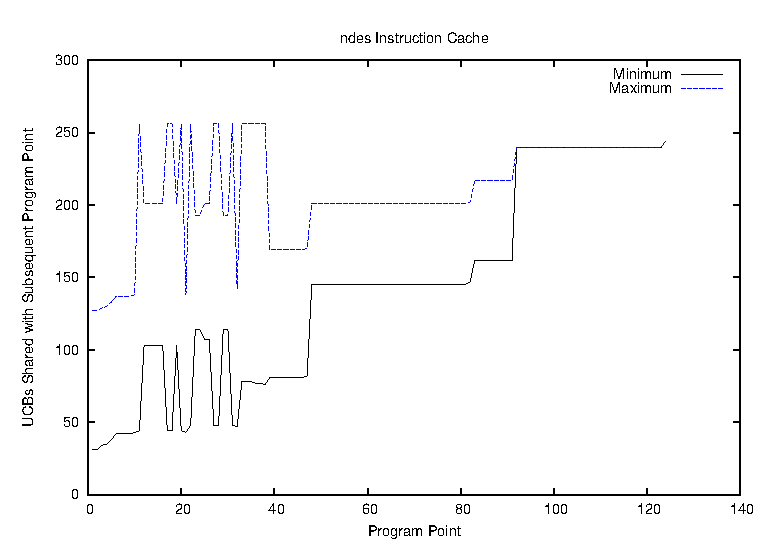
\includegraphics[width=\linewidth]{eps/ndes-icache.eps}
%\caption{NDES Instruction Cache.}
%\label{fig:ndes_instruction_cache}
%\end{center}
%\end{figure}
%
%
% BEGIN:2015-01-31 CT
%
\subsection {Example of LCB Interdependence}\label{sec:example_lcb_interdependence}
%\newline
\indent
To further exemplify the interdependence of preemption points, consider the example shown below.  In order to account for all re-loaded cache blocks (LCBs), preemptions are always included at the first basic block  ${\delta_i^{0}}$ and the last basic block ${\delta_i^{N_i}}$ as shown in Figure~\ref{fig:lcb_ex}.  This is commensurate with the preemptions that occur before and after the task executes.  Assume we have two tasks where ${\tau_2}$ contains four basic blocks which may be preempted by task ${\tau_1}$.  For simplification, assume that the ECBs of task ${\tau_1}$ evicts all UCBs of task ${\tau_2}$.  Let us further assume that we have ${\rho_2 = \{\delta_2^0, \delta_2^1, \delta_2^2, \delta_2^4\}}$.  Using our LCB computation approach, only the re-loaded lines as captured in the terms ${LCB(\delta_2^1, \delta_2^2)}$ and ${LCB(\delta_2^2, \delta_2^4)}$ are included in the ${C_2}$ computation.  ${LCB(\delta_2^0, \delta_2^1)} = 0$ as no LCBs have been cached until after execution of basic block $\delta_2^1$.
%%Note that ${\delta_2^2}$ accesses cache line 3 which may have been present in the cache before task %${\delta_2^0}$ was preempted.  By requiring the inclusion of ${\delta_2^3}$ in ${\rho_2}$ cache line 3 will be %accounted for by ${LCB(\delta_2^1, \delta_2^3)}$. Similarly, the requirement of ${\delta_2^0}$ in ${\rho_2}$ %assures no reloaded cache line is omitted in the calculation of ${C_2}$.

%% \begin{figure}[!htb]
%%   \centering
%%   \def\svgwidth{250pt}
%%   \input{ink/lcb_01.pdf_tex}
%%   \vspace{5pt}
%%   \caption{LCB Interdependence}
%%   \label{fig:test}
%% \end{figure}
%% \begin{figure}[!htb]
%%   \centering
%%   \def\svgwidth{250pt}
%%   \input{ink/lcb_02.pdf_tex}
%%   \vspace{5pt}
%%   \caption{LCB Interdependence}
%%   \label{fig:test_02}
%% \end{figure}

\begin{figure}[!htb]
  \centering
  \def\svgwidth{250pt}
  \input{ink/lcb_03.pdf_tex}
  \vspace{5pt}
  \caption{LCB Interdependence}
  \label{fig:lcb_ex}
\end{figure}

%
% END:2015-01-31 CT
%
